The \CalibrationTool{} class provides methods to calibrate a camera, undistort the camera images using the 
output of the calibration, and save the output into a file. A calibration tool object is created by providing the 
image buffer associated with the camera that is to be calibrated. Table \ref{calibrationtoolmethods} lists 
all methods available in the \CalibrationTool{} class.

\begin{table}[ht]
\caption{Public methods in the \CalibrationTool{} class}
\begin{center}
\begin{tabular}{| l |}
	\hline 
	\multicolumn{1}{| c |}{\CalibrationTool{}} \\
	\hline \hline
	\texttt{start} \\
	\texttt{reset} \\
	\texttt{isCalibrating} \\
	\texttt{calibrate} \\
	\texttt{findAndDrawCorners} \\
	\texttt{addCornersToList} \\
	\texttt{calibrateCamera} \\
	\texttt{initUndistortMap} \\
	\texttt{undistort} \\
	\texttt{setCameraParameters} \\
	\texttt{setChessboardDimensions} \\
	\texttt{setChessboardSquareSize} \\
	\texttt{setRequiredSamples} \\
	\texttt{setWindowDimensions} \\
	\texttt{getCameraParameters} \\
	\texttt{getCameraParametersPath} \\
	\texttt{getChessboardNumberOfColumns} \\
	\texttt{getChessboardNumberOfRows} \\
	\texttt{getChessboardSquareSize} \\
	\texttt{getRequiredSamples} \\
	\texttt{getWindowWidth} \\
	\texttt{getWindowHeight} \\
	\texttt{loadCameraParameters} \\
	\texttt{saveCameraParameters} \\ 
	\texttt{getVectorFromUndistortedCameraImage} \\
	\hline
\end{tabular}
\end{center}
\label{calibrationtoolmethods}
\end{table}

The implementation of the \CalibrationTool{} is based on the calibration functions of the OpenCV open source 
library, which in turn are based on Jean-Yves Bouguet's implementation of Zhang's calibration method
\cite{Bouguet, Zhang}. The calibration process is started by calling the \texttt{start} method, and at any
time it can be restarted by calling \texttt{re\-set} followed by \texttt{start}. The process consists of detecting a 
checkerboard pattern (Figure \ref{checkerboard}) on multiple images until acquiring a preset number of 
calibration images. The information about the position of the checkerboard's corners is extracted from the 
images and then fed to the calibration algorithm. The algorithm for one loop of the calibration process, which 
runs on each user call to the method \texttt{cal\-i\-brate}, is described in Table \ref{calibratealgorithm}.

\begin{figure}[t]
\begin{center}
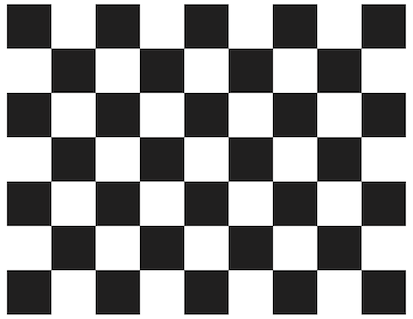
\includegraphics[scale=0.9]{checkerboard.png}
\caption{Checkerboard pattern used for camera calibration}
\label{checkerboard}
\end{center}
\end{figure}

\begin{table}[ht]
\caption{Algorithm for the \texttt{calibrate} method in \CalibrationTool{}}
\begin{center}
\begin{tabular}{ l l }
\hline
\multicolumn{2}{l}{\texttt{CALIBRATE (currentImages, requiredImages):}} \\
1 & \texttt{{\bf If} (currentImages < requiredImages)} \\
2 & \hspace{0.6cm} \texttt{\bf Then:} \\
3 & \hspace{1.2cm} \texttt{Search checkerboard pattern in the image;} \\
4 & \hspace{1.2cm} \texttt{{\bf If} the pattern is found} \\
5 & \hspace{1.8cm} \texttt{\bf Then:} \\
6 & \hspace{2.4cm} \texttt{Extract the corners and save them;} \\
7 & \hspace{2.4cm} \texttt{Increment currentImages counter;} \\
8 & \hspace{0.6cm} \texttt{\bf Else:} \\
9 & \hspace{1.2cm} \texttt{Run calibration algorithm with saved corners;} \\
\hline
\end{tabular}
\end{center}
\label{calibratealgorithm}
\end{table}

The algorithm starts by checking if the count of acquired images is less than the number of required images.
If it is, it calls the \texttt{find\-And\-Draw\-Cor\-ners} method to search the image for the position of the 
calibration pattern's corners (line 3). If the complete set of corners is found, \texttt{add\-Cor\-ners\-To\-List} is 
called in order to save their positions into a list (line 6), and then the count of acquired images is incremented
(line 7). Therefore, the user must call \texttt{cal\-i\-brate} until the number of acquired images reaches 
the number of required images. Once it reaches it, an additional call to \texttt{cal\-i\-brate} runs the camera 
calibration algorithm by calling the \texttt{cal\-i\-brate\-Cam\-er\-a} method (line 9). At any point of the 
calibration process the user can call \texttt{is\-Cal\-i\-brat\-ing} to check if the calibration tool is waiting for 
more images.

Once the camera calibration is performed, the results are saved into an object of type \CameraParameters{}
which is accessed through the \texttt{get\-Cam\-e\-ra\-Pa\-ram\-e\-ters} method. This object holds the 
intrinsic parameters (focal length, principal point, distortion coefficients) and extrinsic parameters 
(rotation and translation vectors) that describe the camera. The camera parameters can be saved into 
or read from an XML file using the \texttt{save\-Cam\-er\-aPa\-ram\-e\-ters} and 
\texttt{load\-Cam\-er\-a\-Pa\-ram\-e\-ters} methods, respectively. 

Finally, the \CalibrationTool{} class provides the methods to undistort the camera images given the camera's
parameters values. First, the x-coordinate and y-coordinate pixel undistortion maps need to be created by 
calling the \texttt{in\-it\-Un\-dis\-tort\-Map} method. This method assumes that the camera parameters object 
has been set, either by running the calibration process, loading the parameters from a file, or setting the 
object using the \texttt{set\-Cam\-er\-a\-Pa\-ram\-e\-ters} method. After initializing the undistortion maps, 
each call to the \texttt{un\-dis\-tort} method will undistort the image in the calibration tool's image buffer.


